\chapter{Methods}

\epigraph{``It is not unscientific to make a guess, although many people who are not in science think it is."}{\textit{R. P. Feynman}}

In order for symbolic extraction to take place in a DSRL system, the latent space must preserve the types of objects and the spatial information of the original scene. In other words, from the latent space alone, it must be possible to deduce an object's type and location. We explore the feasibility of using fully-convolutional variational autoencoders for this purpose. This is exciting new territory; the fully-convolutional variational autoencoder has (to the best of our knowledge) never been explored. We therefore have many degrees of freedom with how we proceed. In this section, we will make educated guesses of how a working architecture would look and the encoding of desirable properties in loss functions, which will be inspired by the successful techniques developed in $\beta$-VAE.


\label{ch:methods}


%
%
%
%
%
\section{Single Latent Filter}

As mentioned, the type and position of an object must be preserved in the latent space. This may be achieved by using a single latent filter, with the object type corresponding to the value of the activation at the relevant position on the filter. Recall that it does not make sense to use an activation function in the latent space, and therefore the object type is represented by an unbounded real number.


%
%
\subsection{Architecture}
The input image is passed through convolutional layers to build increasingly meaningful hidden representations. The convolutional mean $\vec{\mu}$ and variance $\vec{\sigma}^2$, both of shape $(1, m, n)$, are sampled using the reparameterisation trick
\begin{align}
\vec{z} = g_{\vec{\phi}}(\vec{x}, \vec{\epsilon}) = \vec{\mu} + \vec{\sigma} \odot \vec{\epsilon} \quad\quad\quad \vec{\epsilon} \sim \mathcal{N}(\vec{0}, \vec{I})
\tag{\ref{eq:reparameterisation_trick}}
\end{align}
so we may use backpropagation. The corresponding deconvolutional layers are applied to reconstruct the original image.\\

\begin{figure}[H]
\centering
\captionsetup{justification=centering}
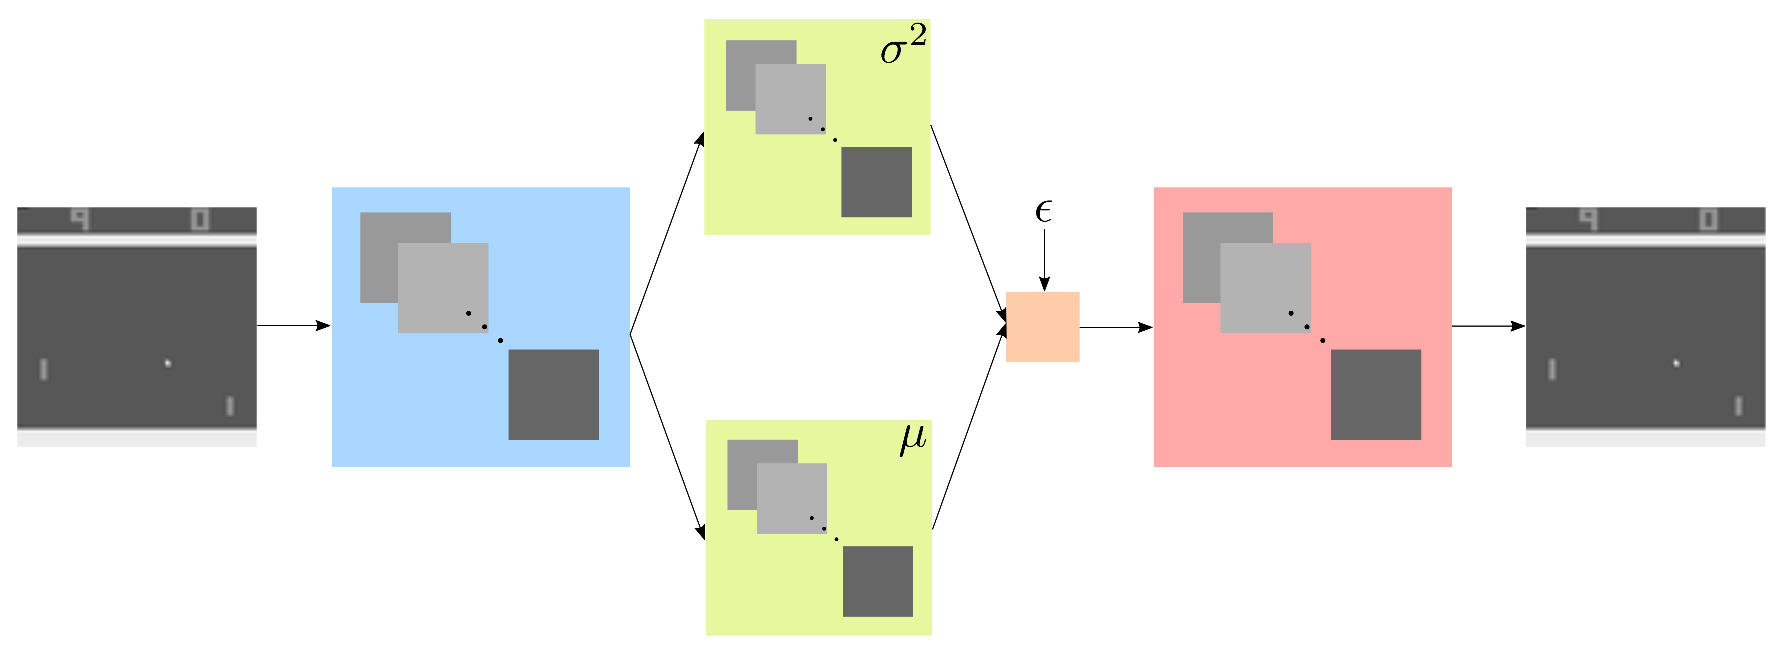
\includegraphics[scale=0.6]{methods/latent_image_architecture.eps}
\caption{The fully-convolutional single latent filter architecture. \textbf{Blue:} An arbitrary amount of convolutional layers. \textbf{Green:} The latent mean $\vec{\mu}$ and variance $\vec{\sigma}^2$, which are both single filters of shape $(1, m, n)$. \textbf{Orange:} A single latent filter of shape $(1, m, n)$ sampled component-wise from $\vec{\mu}$ and $\vec{\sigma}^2$. \textbf{Red:} The corresponding deconvolutional layers.}
\label{fig:latent_image_architecture}
\end{figure}

%
%
\subsection{Neuron-Level Decoupling}
As with all autoencoders, a reconstruction loss term must appear in the loss function as to learn the identity function, which ensures a meaningful lower-dimensional representation is learnt in the latent space. Hence we also include this term in the final loss function for this architecture.

We also saw in $\beta$-VAE that the multiplicative factor on the KL loss term varies the pressure of redundancy reduction on the latent space. As we seek to have non-zero activations in the latent space if and only if an object is present, it's in our interest to reduce the number of unnecessarily activated neurons. Therefore the application of a redundancy pressure term seems suitable, and is therefore included in the loss function. However, as we no longer have a one-dimensional latent space, we must decide on how this term will appropriately reduce redundancy in a two-dimensional latent space.

To reduce the redundancy in a two-dimensional latent space, we choose to flatten the $(1, m, n)$-dimensional single latent filter to an $m \times n$ vector, which is then matched to an isotropic Gaussian. We choose this isotropic Gaussian to be $\mathcal{N}(\vec{0}, \vec{I})$ for convenience.

\begin{align}
\mathcal{L}(\vec{\theta}, \vec{\phi}; \vec{x}) = -D_{KL}(q_{\vec{\phi}}(\vec{z}|\vec{x}) || p_{\vec{\theta}}(\vec{z})) + \mathbf{E}_{q_{\vec{\phi}}(\vec{z}|\vec{x})}\big[\log p_{\vec{\theta}}(\vec{x} | \vec{z}) \big]
\tag{\ref{eq:elbo_kl_loss_plus_expectation}}
\end{align}


\begin{itemize}
\item As with the variational autoencoders seen earlier, we have a reconstruction loss term in the loss function
\item Learning the identity function ensures a meaningful lower-dimensional representation is learnt in the latent space
\item However, as we only want values of high magnitude where there are objects, we need to reduce the reundancy in the latent space
\item Therefore we need to decide on the appropriate term in the loss function to reduce redundancy
\item The latent filter of shape $(1, m, n)$ is flattened to a $m \times n$ vector
\item This flattened representation of the single latent filter is used then pressured to be close to an isotropic Gaussian with KL divergence ...equation here...
\item This pressuring reduces redundancy in the latent space as if neighbouring pixels 
\end{itemize}

\begin{figure}[H]
\centering
\captionsetup{justification=centering}
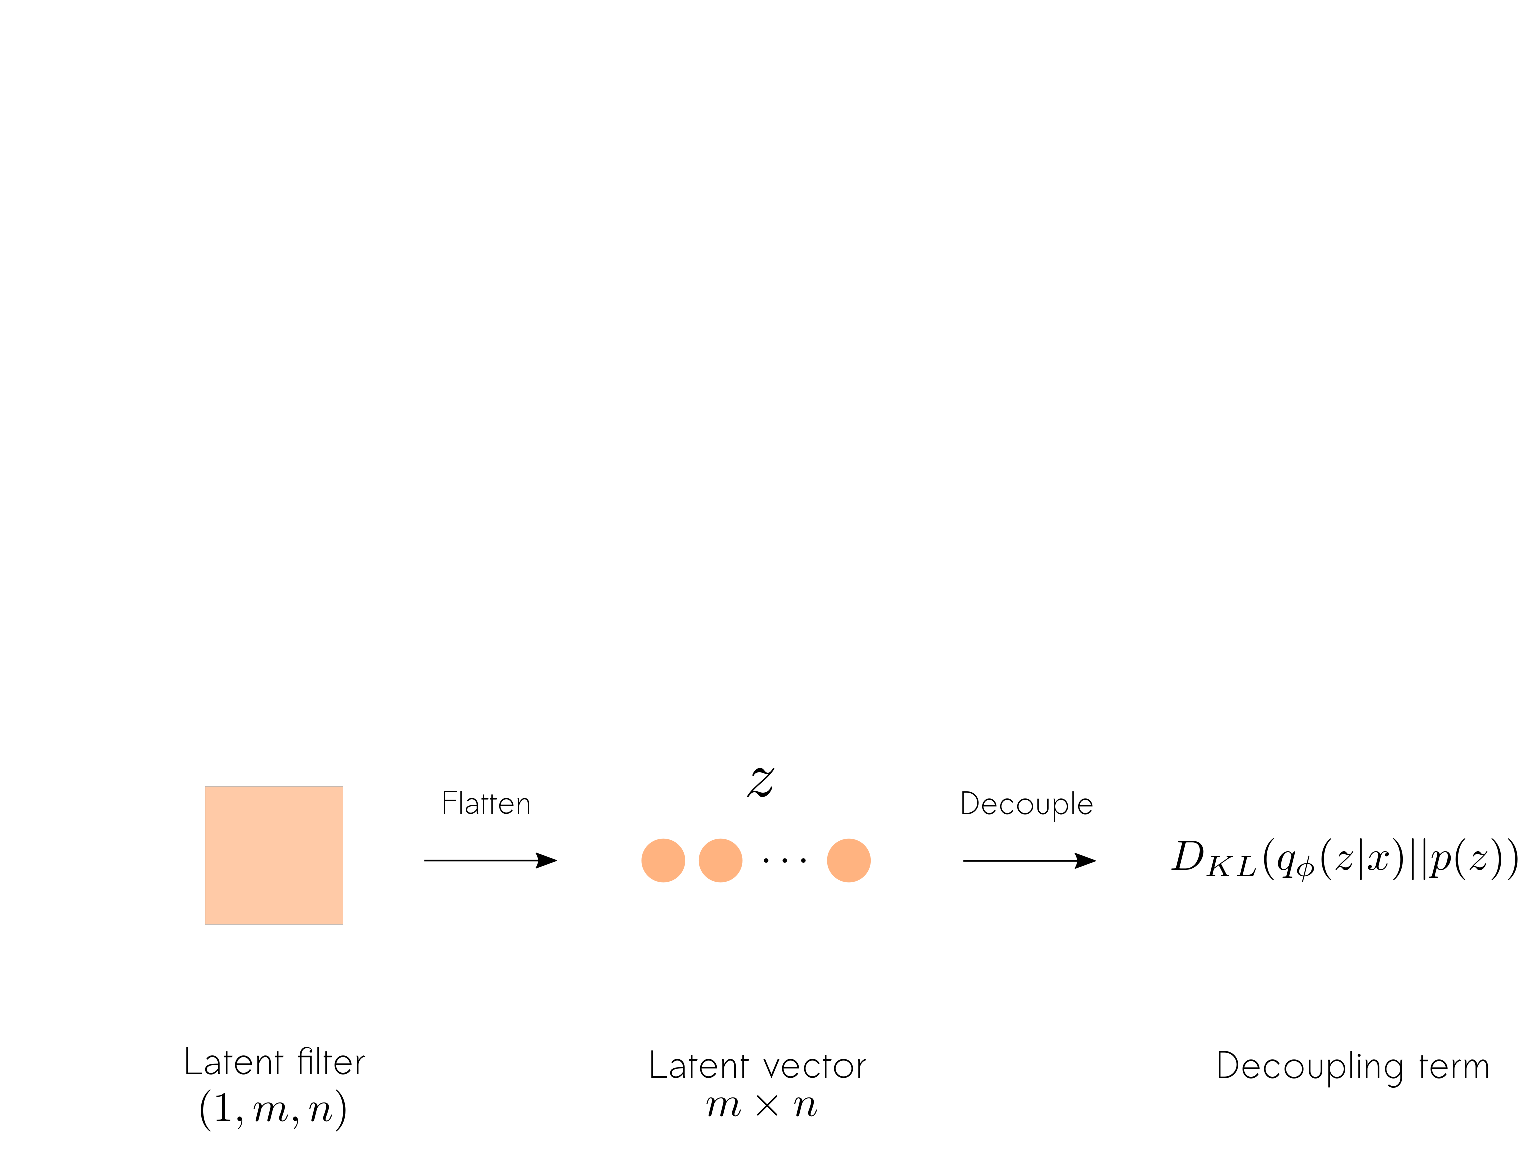
\includegraphics[scale=0.6]{methods/latent_image_flattening_latent_space.eps}
\caption{Caption.}
\label{fig:latent_image_flattening_latent_space}
\end{figure}


%
%
%
%
%
\section{Multiple Latent Filters}
\begin{itemize}
\item As mentioned, a single latent filter seems unlikely to be able to represent a types of objects in the original scene
\item This leads to the idea of pressuring filters to learn at most one object type
\item For scenes with more than one object type, the latent space must have multiple features
\end{itemize}
%
%
\subsection{Architecture}
TODO: Finish subsection

\begin{itemize}
\item The architecture is the same as the fully-convolutional single lantent filter architecture, but with one difference in the latent space.
\item The convolutional mean $\vec{\mu}$ and variance $\vec{\sigma}^2$, both of shape $(k, m, n)$, are sampled using ... cite reparameterisation trick here... (so we may use backpropagation) to give the latent space of shape $(k, m, n)$. 
\item The proposed architecture is shown in Figure (\ref{fig:decoupling_indiscriminately_horizontal})
\end{itemize}

\begin{figure}[h!]
\centering
\captionsetup{justification=centering}
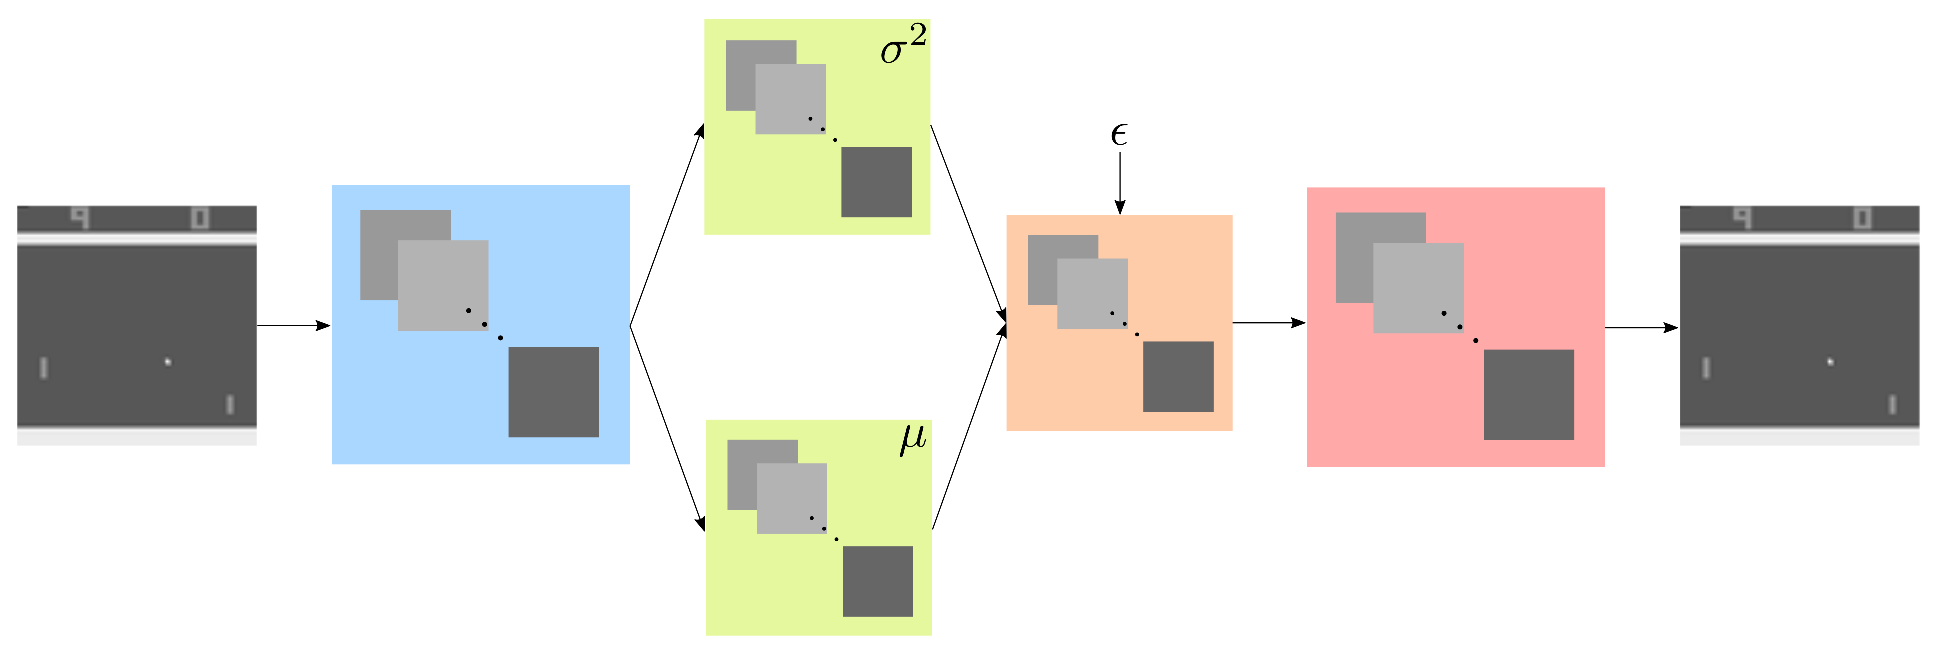
\includegraphics[scale=0.55]{methods/decoupling_indiscriminately_horizontal.eps}
\caption{The fully-convolutional multiple latent filter architecture. \textbf{Blue:} Unchanged. \textbf{Green:} The latent mean $\vec{\mu}$ and variance $\vec{\sigma}^2$, which are both single filters of shape $(k, m, n)$. \textbf{Orange:} A single latent filter of shape $(k, m, n)$ sampled component-wise from $\vec{\mu}$ and $\vec{\sigma}^2$. \textbf{Red:} Unchanged.}
\label{fig:decoupling_indiscriminately_horizontal}
\end{figure}


\begin{itemize}
\item By the same reasoning for the previous architecture, we keep the reconstruction loss term. 
\item Need to decide on the appropriate term in the loss function to reduce redundancy
\item Here some creativity is needed on how to reduce redundancy over the filters
\item We present three methods of decoupling the latent volume: ...list...
\end{itemize}

%
%
\subsection{Neuron-Level Decoupling}
\begin{itemize}
\item The latent filter of shape $(k, m, n)$ is flattened to a $k \times m \times n$ vector
\item This flattened representation of the single latent filter is used then pressured to be close to an isotropic Gaussian with KL divergence ...equation here...
\item This pressuring reduces redundancy among all pixels in the latent volume
\item The loss function can therefore be written as ...loss function...
\end{itemize}

\begin{figure}[H]
\centering
\captionsetup{justification=centering}
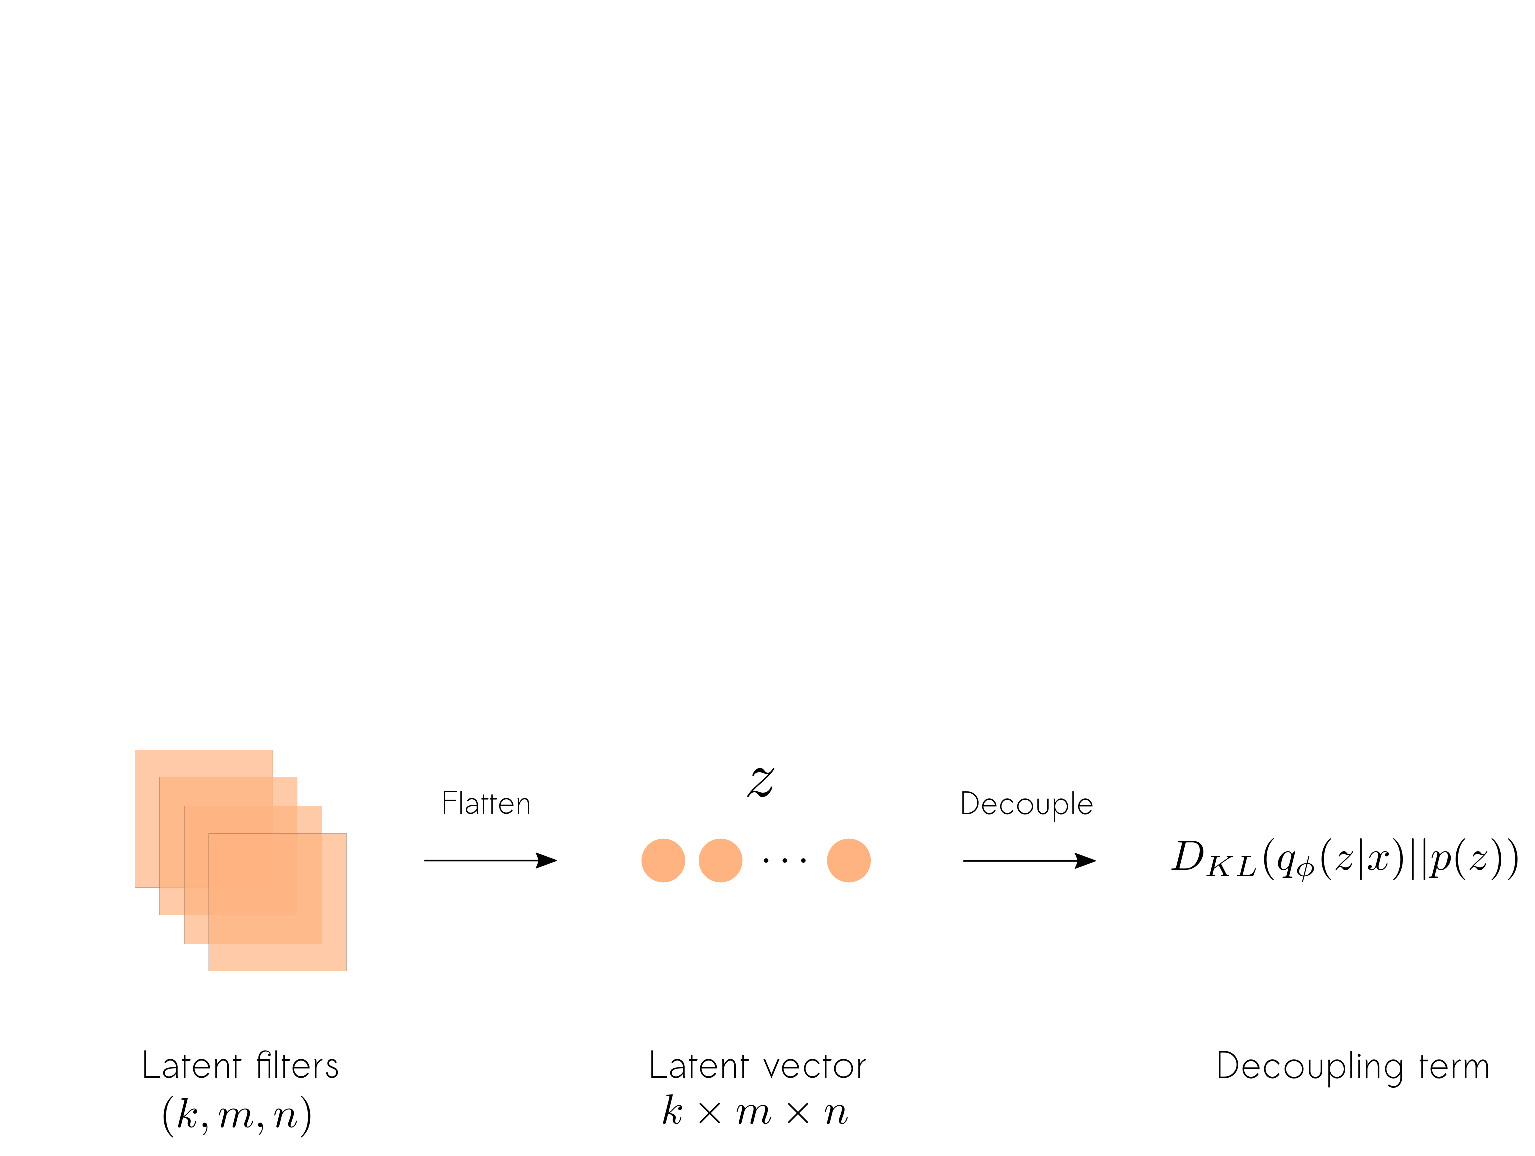
\includegraphics[scale=0.6]{methods/decoupling_indiscriminately_flattening_latent_space.eps}
\caption{Caption.}
\label{fig:decoupling_indiscriminately_flattening_latent_space}
\end{figure}

%
%
\subsection{Na{\"i}ve Filter-Level Decoupling}
\begin{itemize}
\item The $k$ filters of the $(k, m, n)$-dimensional latent space are averaged across their activations and stored in a vector $\bar{\vec{z}}$
\item We've reduced our problem to one solved in $\beta$-VAE!
\item To disentangle the average activations over filters, we pressure the vector $\bar{\vec{z}}$ to be close to an isotropic Gaussian
\item This pressuring reduces redundancy the average activations among filters
\item This achieves the desired outcome because: - if two filters that have learnt the same object type, one may be pressured to match the prior (or ``forgotten"), as the same information about the original scene is encoded in the latent space
\item The loss function then can be written as ...loss function...
\end{itemize}

\begin{figure}[H]
\centering
\captionsetup{justification=centering}
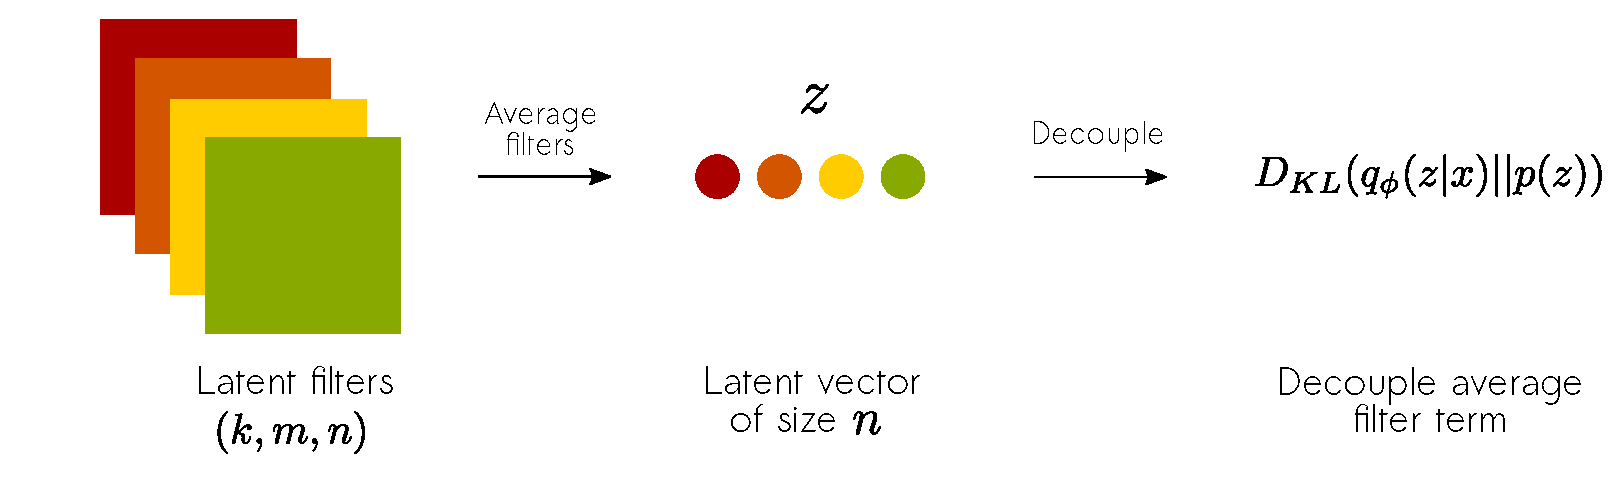
\includegraphics[scale=0.6]{methods/decoupling_averages_latent_space.eps}
\caption{Caption.}
\label{fig:decoupling_averages_latent_space}
\end{figure}

%
%
\subsection{Weighted Filter-Level Decoupling}

\begin{itemize}
\item Before we have taken the sum of the pixel-wise loss using binary cross entropy and the sum of the average activations  over latent filters
\item This may be a bad design choice, as the KL loss is extremely small compared to the reconstruction loss
\item For example, suppose we use an input image of $28 \times 28$ and $16$ latent filters. Further assume that, on average, the reconstruction loss of one pixel is $0.5$ and the average activation is $4$ (both are reasonable for the MNIST data set). Then the reconstruction loss is 28 * 28 * 0.5 = 392 compared to the KL loss of 16 * 2 = 32 - approximately an order of magnitude difference.
\item Instead, if we weight the average binary cross entropy and average filter activations by the number of pixels taking in the respective averages, we may get a more balanced loss function 
\item Therefore our final loss function is ...
\end{itemize}

\begin{figure}[H]
\centering
\captionsetup{justification=centering}
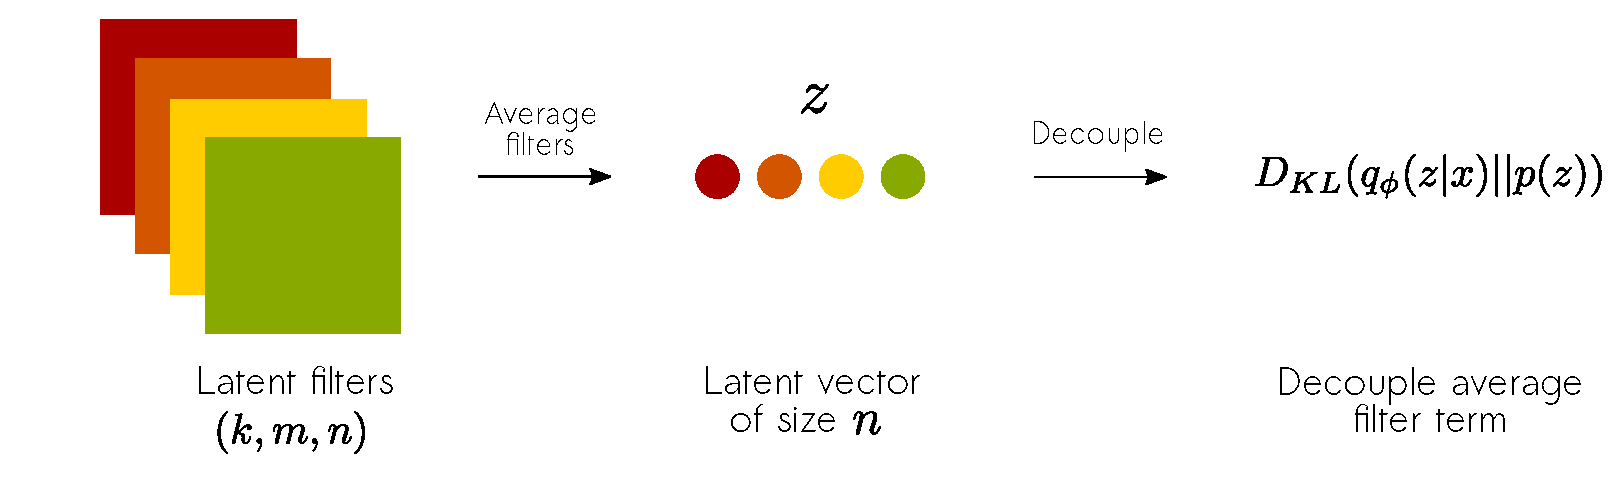
\includegraphics[scale=0.6]{methods/decoupling_averages_latent_space.eps}
\caption{Caption.}
\label{fig:decoupling_averages_latent_space}
\end{figure}


%
%
%
%
%
\section{Separating Colour Spaces}

\begin{itemize}
\item As the task of unsupervised object recognition in fully-convolutional variational autoencoders is an open problem, it's reasonable to start by solving easy recognition tasks
\item Since sprites are of different colours in Atari games, maybe we could leverage this property by including the colour channels of the frame as input to make the separation of objects easier
\item An example for a frame of Space Invaders is shown in Figure (\ref{fig:separating_colour_spaces})
\item This technique may be applied to all architectures listed here.
\end{itemize}

\begin{figure}[h!]
\centering
\captionsetup{justification=centering}
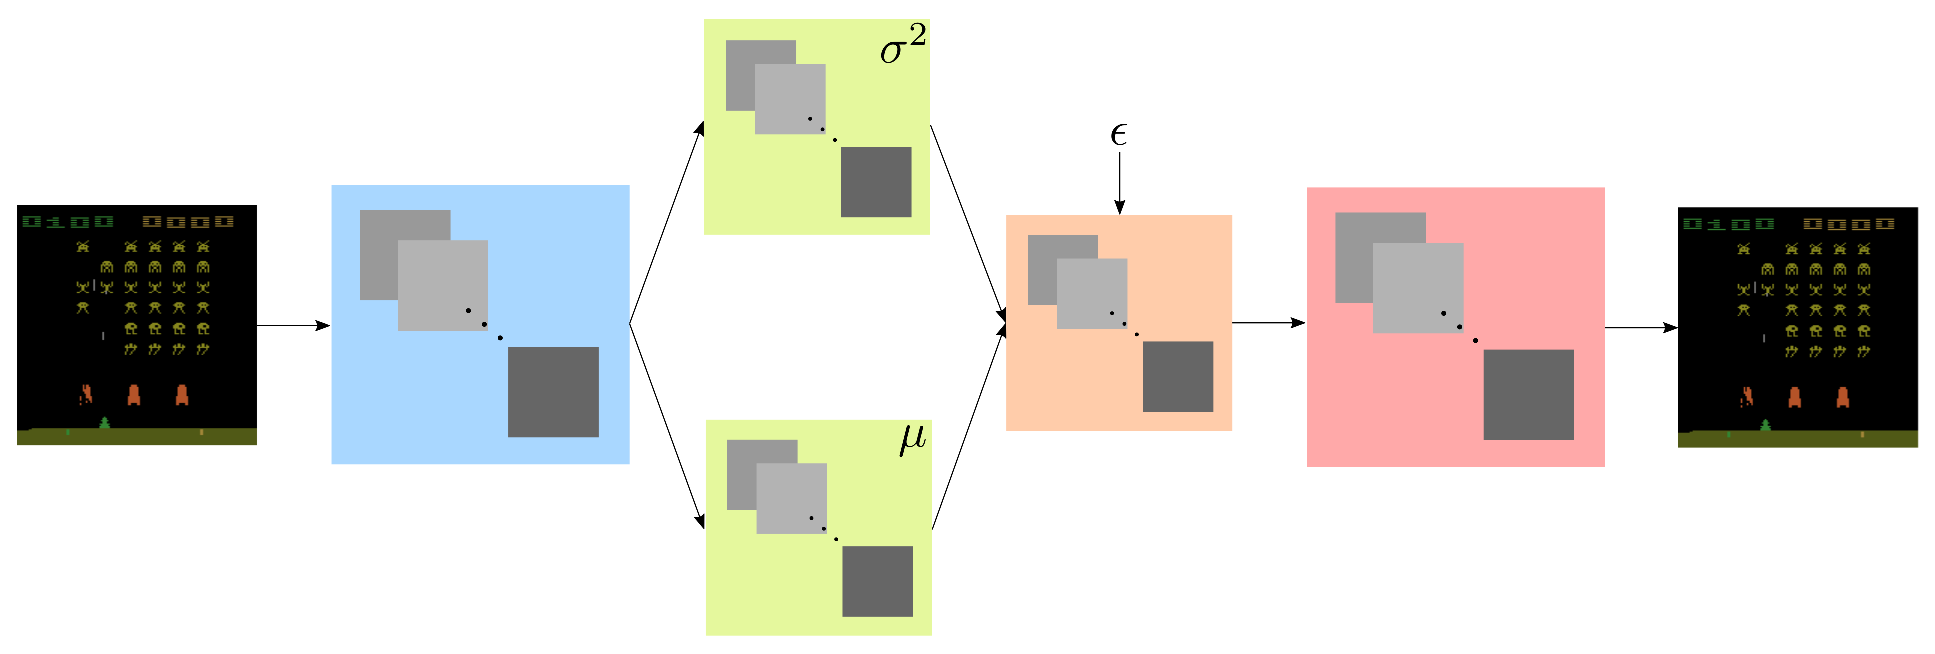
\includegraphics[scale=0.55]{methods/separating_colour_spaces_architecture.eps}
\caption{Caption.}
\label{fig:separating_colour_spaces_architecture}
\end{figure}

\begin{figure*}[h!]
\centering
\captionsetup{justification=centering}
\begin{multicols}{4}
    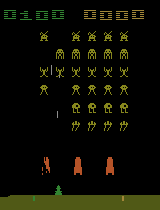
\includegraphics[scale=0.7]{figures/methods/separating_colour_spaces_original.png}
    \caption{Original}\par
    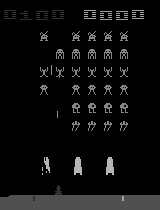
\includegraphics[scale=0.7]{figures/methods/separating_colour_spaces_r.png}
    \caption{Red}\par
    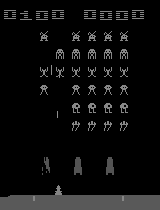
\includegraphics[scale=0.7]{figures/methods/separating_colour_spaces_g.png}
    \caption{Green}\par
    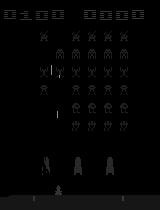
\includegraphics[scale=0.7]{figures/methods/separating_colour_spaces_b.png}
    \caption{Blue}
\end{multicols}
\caption{A comparison of a $210 \times 160$ RGB frame from Space Invaders and its red, green and blue channels. The bullet is clearly separated from other sprites in the blue channel. The red and green channels separate collections of sprites. The red channel excludes the gunship and players score, while the green partially excludes the barriers.}
\label{fig:separating_colour_spaces}
\end{figure*}

\begin{itemize}

\item Even if we saw perfect separation of sprites in colour spaces, we'd only be able to exclusively separate at most three object types
\end{itemize}



%
%
%
%
%
\section{Winner Takes All}

\begin{itemize}
\item As mentioned, it seems likely that objects may be classified by which latent filter has a high activation in its position
\item Assuming the latent space takes this structure, we would expect no more than one filter to be activated in any given position.
\item In other words, objects must have distinct types: a sprite cannot be a gunship and a number at the same time.
\item This leads to the Winner Takes All method, where we apply a position-wise pressure to the latent space so that no more than one filter has a high activation in any given position.
\item Naturally this applies to fully-convolutional multiple latent filter architectures.
\end{itemize}


\begin{figure*}[h!]
\centering
\captionsetup{justification=centering}
\begin{multicols}{2}
    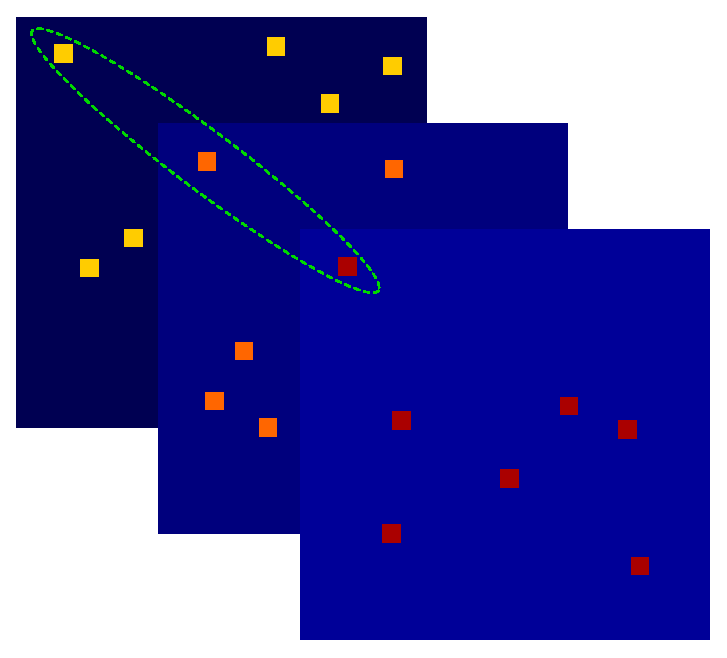
\includegraphics[scale=0.4]{figures/methods/winner_takes_all_object_on_every_filter.eps}
    \caption{Multiple types of objects recognised in same position.}
    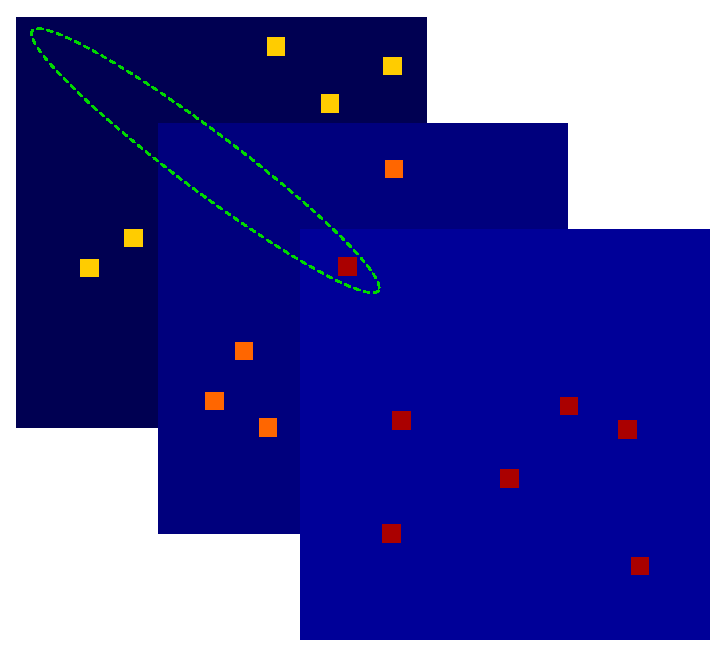
\includegraphics[scale=0.4]{figures/methods/winner_takes_all_object_on_one_filter.eps}
    \caption{At most one object recognised in a given position.}
\end{multicols}
\caption{Caption.}
\label{fig:winner_takes_all_activations_on_layers}
\end{figure*}


\subsection{Derivation}

We wish to include a term in our loss function that ensures no more than one filter has a high activation in any given position.

Consider a convolutional latent space $\vec{z}$ of shape $(k, m, n)$. Let $\vec{z}^{i,j} \in \mathbb{R}^k$ be the vector storing the activations over the $k$ filters at position $(i, j)$. Naturally, we also let $q_{\vec{\phi}}^{i, j}(\vec{z} | \vec{x})$ represent the probabilistic encoder for $\vec{z}^{i,j}\in \mathbb{R}^k$. By matching the probabilistic encoder to an isotropic Gaussian we may reduce the redundancy, as argued previously. We choose to include the following term in our loss function:

\begin{align}
\sum_{i=1}^m \sum_{j=1}^n D_{KL}(q_{\vec{\phi}}^{i, j}(\vec{z} | \vec{x}) || p^{i,j}(\vec{z}))  \quad \textup{ where } \quad p^{i,j}(\vec{z}) = \mathcal{N}(\vec{0}, \vec{I})
\end{align}

As shown with $\beta$-VAE, the multiplicative $\beta$ controls the redundancy pressure. We will include this also and see if we observe a similar effect later.

\begin{figure}[h!]
\centering
\captionsetup{justification=centering}
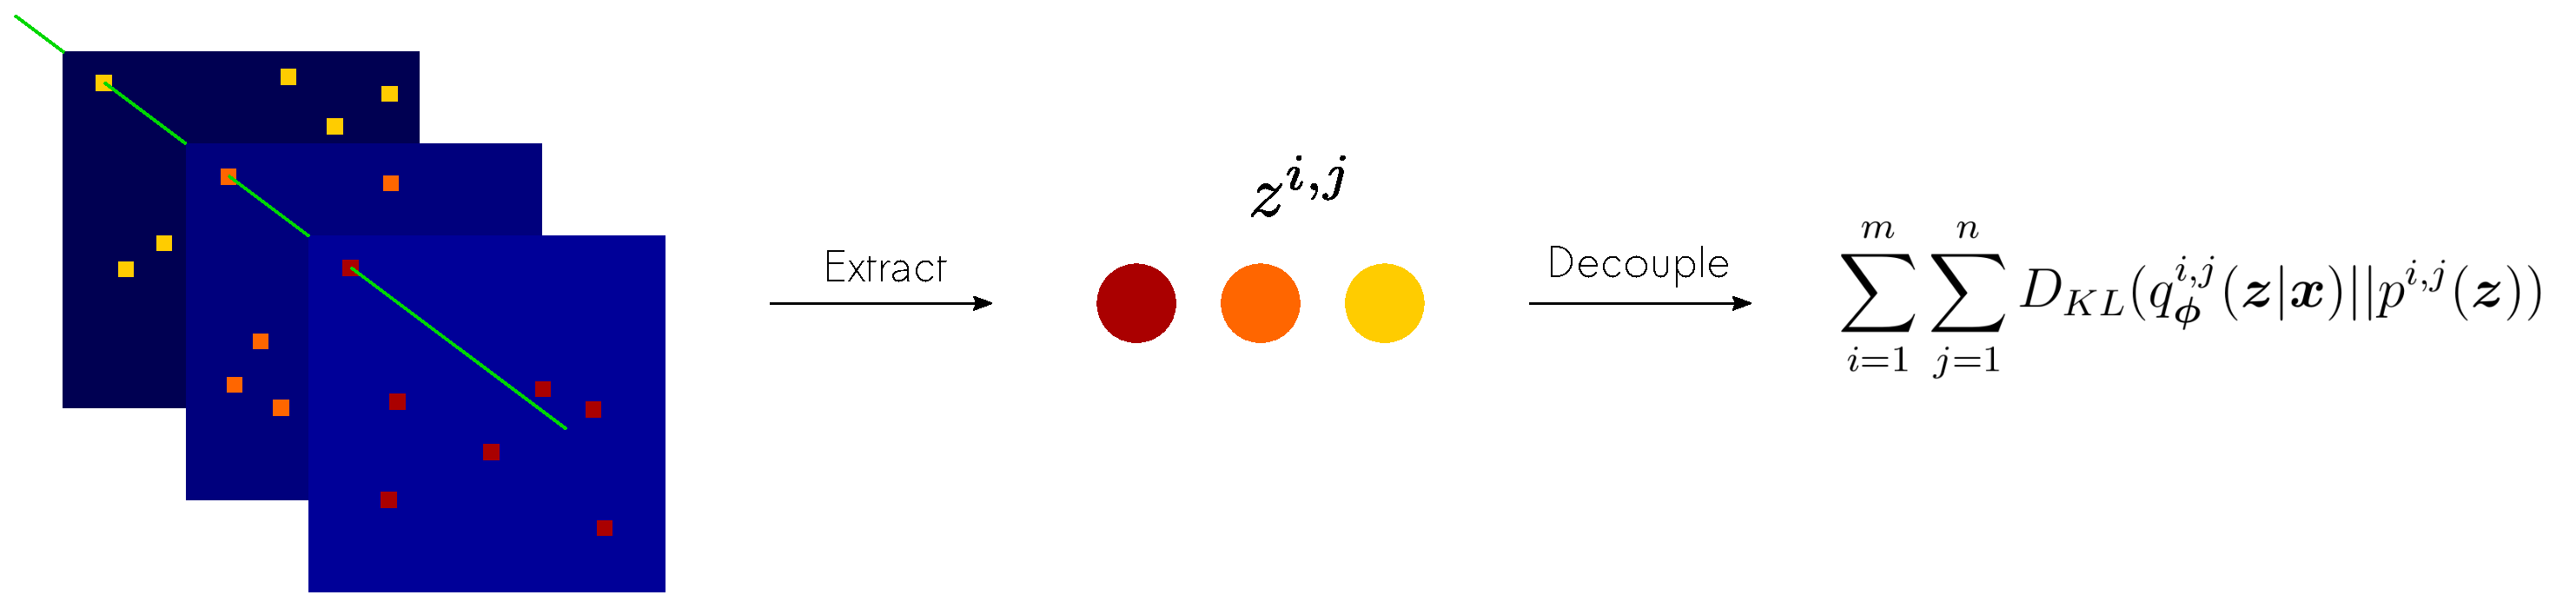
\includegraphics[scale=0.3]{methods/winner_takes_all_line_through_object_on_every_filter_flow_chart.eps}
\label{fig:winner_takes_all_line_through_object_on_every_filter}
\end{figure}

Therefore the final loss function is given as:

\begin{align}
\mathcal{L}_{WTA}(\vec{\theta}, \vec{\phi}; \vec{x}) = \mathbf{E}_{q_{\vec{\phi}}(\vec{z} | \vec{x})} \big[ \log p_{\vec{\theta}}(\vec{x} | \vec{z}) \big] - \beta \sum_{i=1}^m \sum_{j=1}^n D_{KL}(q_{\vec{\phi}}^{i, j}(\vec{z} | \vec{x}) || p^{i,j}(\vec{z})) 
\end{align}


%
%
%
%
%
\section{Orthogonal Convolutions}
\lipsum[2]
\subsection{Architecture}
TODO: Finish subsection
\begin{figure}[h!]
\centering
\captionsetup{justification=centering}
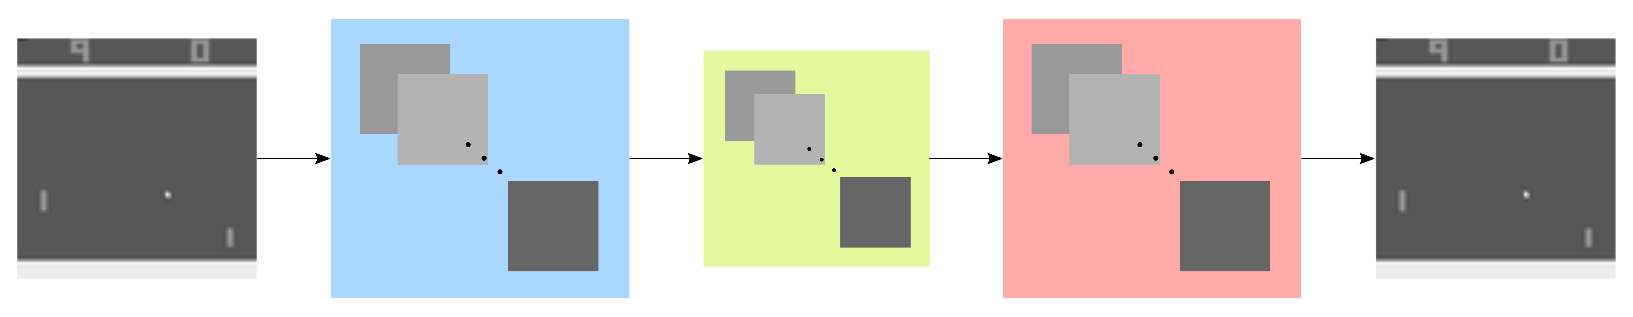
\includegraphics[scale=0.63]{methods/orthogonal_convolutions_archiecture.eps}
\caption{Caption.}
\label{fig:orthogonal_convolutions_archiecture}
\end{figure}

\subsection{Derivation}
TODO: Finish subsection